\documentclass[11pt]{beamer}
\usepackage[spanish]{babel}
\usetheme{Dresden}
\usepackage[utf8]{inputenc}
\usepackage{amsmath}
\usepackage{amsfonts}
\usepackage{amssymb}
\usepackage{graphicx}
\usepackage{url}
\usepackage{bbding}
\usepackage[all]{xy}
\usepackage{tikz}

\usetikzlibrary{arrows,automata, shapes.arrows, shapes.geometric,shapes, calc}
\tikzstyle{vertex}=[draw,fill=black!15,ellipse,minimum size=20pt,inner sep=0pt]
\tikzstyle{terminal}=[draw,fill=blue!15,rectangle,minimum size=20pt,inner sep=1pt]
\tikzstyle{terminal1}=[draw,fill=blue!15,rectangle,minimum size=10pt,inner sep=0pt]
\tikzstyle{vacio}=[draw,fill=black!15,circle,minimum size=0pt,inner sep=0pt]

\author{Edgar Andrade, Ph.D.}
\title{Lógica e Inteligencia Artificial}
\subtitle{Resolución de problemas}
%\setbeamercovered{transparent} 
%\setbeamertemplate{navigation symbols}{} 
\logo{
\includegraphics[scale=.15]{imagenes/Macc.png}} 
\institute{Matemáticas Aplicadas y Ciencias de la computación} 
\date{Última revisión: Febrero 2021} 
%\subject{} 
\begin{document}

\begin{frame}
\titlepage
\end{frame}

\begin{frame}
\tableofcontents
\end{frame}

\AtBeginSection[]
  {
     \begin{frame}<beamer>
     \frametitle{Contenido}
     \tableofcontents[currentsection]
     \end{frame}
  }

\section{Motivación}

\begin{frame}{Inteligencia de máquina}

\begin{block}{Aspiraciones}

\

``Turing pensaba que había llegado el momento de que los filósofos, los matemáticos y los científicos se tomaran en serio el hecho de que los \textbf{computadores} no eran simples motores de cálculo, sino que \textbf{eran capaces de un comportamiento que debía considerarse inteligente}.'' 

\begin{flushright}
(Robin Gandy)
\end{flushright}
\end{block}

\end{frame}

\begin{frame}{Ajedrez e IA}

\begin{minipage}{0.5\linewidth}
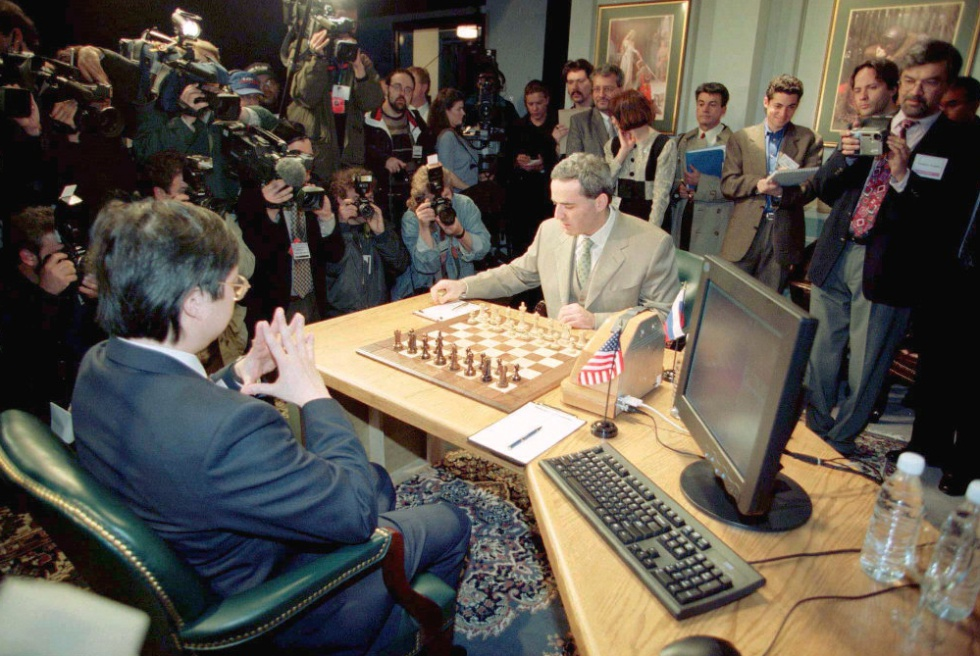
\includegraphics[scale=0.1]{imagenes/kasparov_vs_deep_blue}

\

El Ajedrez es la ``drosofila\par de la Inteligencia Artificial''

\begin{flushright}
John McCarthy (1990)
\end{flushright}

\begin{tiny}
\url{https://fast-poll.com/poll/b5363a36}
\end{tiny}

\end{minipage}\begin{minipage}{0.5\linewidth}

\vspace*{-2\baselineskip}

\visible<2->{
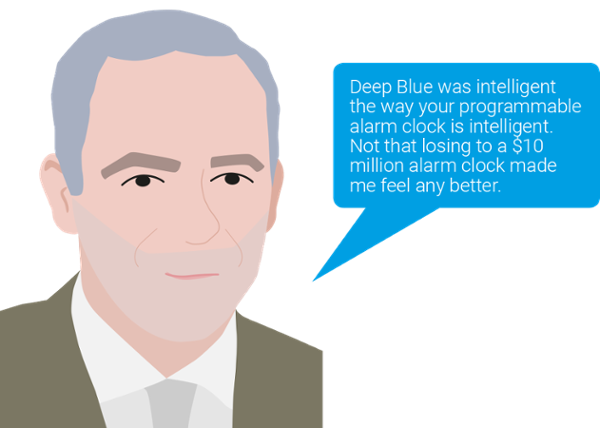
\includegraphics[scale=0.25]{imagenes/Kasparov_on_chess_ia}
}

\

\visible<3->{
\hspace{0.5cm}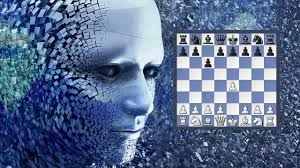
\includegraphics[scale=0.4]{imagenes/alpha_zero}
}

\end{minipage}

\end{frame}


\begin{frame}{El juego de la imitación}

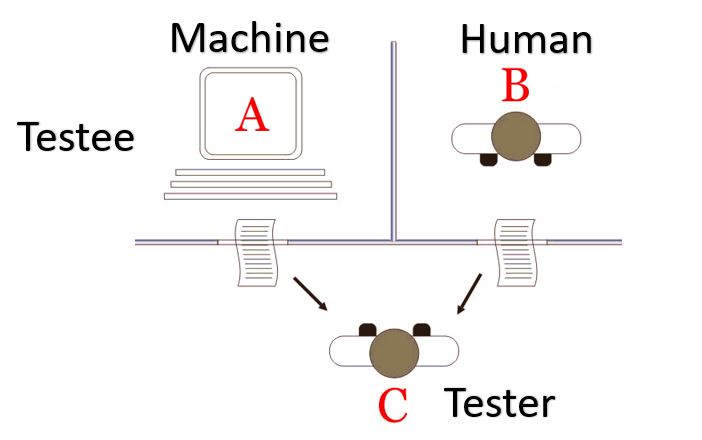
\includegraphics[scale=.5]{imagenes/turing-test.jpg}

\end{frame}


\section{¿Qué es la IA?}

\begin{frame}{Ejes definitorios}

\begin{center}
\begin{tabular}{ccc}
\textbf{Objeto de desempeño} & \hspace{1cm} & \textbf{Tipo de desempeño}\\
\\
\visible<2->{\alert<4,6>{Pensamientos}} && \visible<3->{\alert<4-5>{Humano}}\\
\\
\visible<2->{\alert<5,7>{Acciones}} && \visible<3->{\alert<6-7>{Óptimo}}\\

\end{tabular}
\end{center}

\only<4>{
\begin{block}{Primera alternativa}
Construir máquinas que piensan como un ser humano
\end{block}

\

Fast poll: ¿Es posible alcanzar la primera alternativa?

\url{https://fast-poll.com/poll/d8f0eef4}

}

\only<5>{
\begin{block}{Segunda alternativa}
Construir máquinas que actúan como un ser humano
\end{block}
}

\only<6>{
\begin{block}{Tercera alternativa}
Construir máquinas que piensan de manera óptima
\end{block}
}

\only<7>{
\begin{block}{Cuarta alternativa}
Construir máquinas que actúan de manera óptima
\end{block}
}

\end{frame}

\section{Momentos históricos}

\begin{frame}{Gestación (1670-1955)}

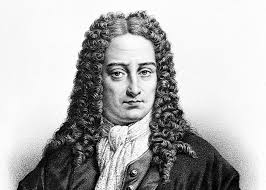
\includegraphics[scale=.45]{imagenes/Leibniz}\hspace{0.8cm}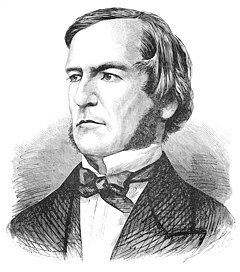
\includegraphics[scale=.3]{imagenes/Boole}\hspace{0.8cm}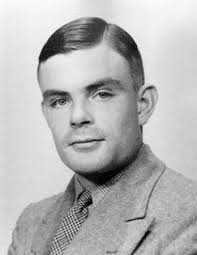
\includegraphics[scale=.35]{imagenes/turing}

\end{frame}


\begin{frame}{Nacimiento (1956)}

\begin{minipage}{.45\linewidth}

\begin{center}

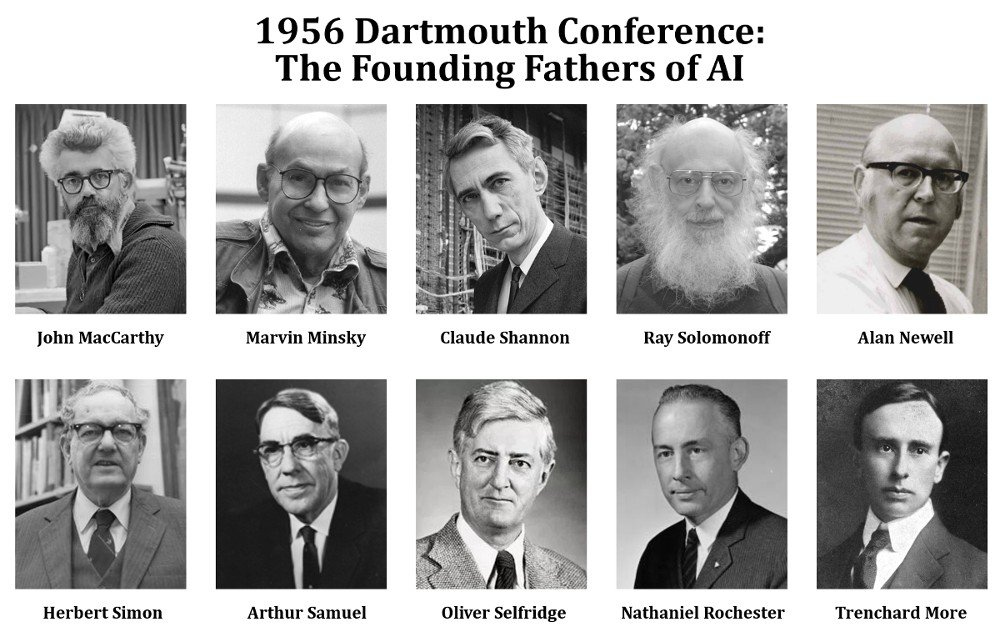
\includegraphics[scale=.15]{imagenes/darmouth_conference.png}

\end{center}

\end{minipage}\hspace{0.5cm}\begin{minipage}{.5\linewidth}

\begin{center}

1956 MIT Conference

\

\includegraphics[scale=.17]{imagenes/Chomsky}\hspace{0.4cm}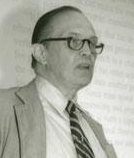
\includegraphics[scale=.28]{imagenes/Miller}

\end{center}

\end{minipage}

\end{frame}


\begin{frame}{Entusiasmo inicial (1952-1969)}

\begin{minipage}{.45\linewidth}

\begin{enumerate}
\item Demostración automática de teoremas
\item Juego de Damas
\item Micromundos
\end{enumerate}

\end{minipage}\hspace{.5cm}\begin{minipage}{.5\linewidth}

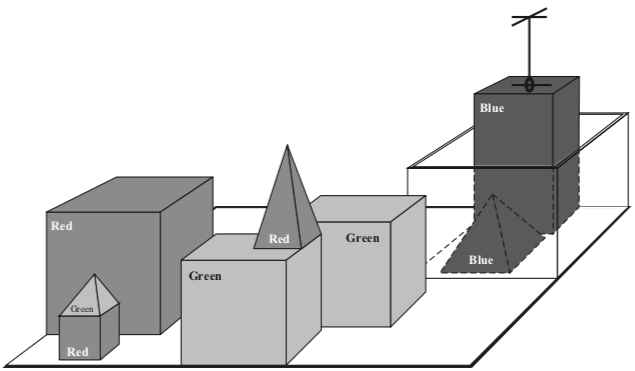
\includegraphics[scale=.2]{imagenes/micromundos}

\end{minipage}


\end{frame}


\begin{frame}{Otros momentos importantes}

\begin{itemize}
\item  Sistemas basados en conocimiento (1969-1986)
\item El regreso de las redes neuronales (1986-presente)
\item Big data (2001-presente)
\end{itemize}

\end{frame}


\section{Agentes y entornos}

\begin{frame}{Task environments}

\begin{minipage}{.5\linewidth}

La IA no es un alma perdida en un universo vacío. Más bien, el objetivo aquí es construir un agente que percibe y actua en un entorno para atender una tarea concreta.

\end{minipage}\hspace{.1\linewidth}\begin{minipage}{.4\linewidth}

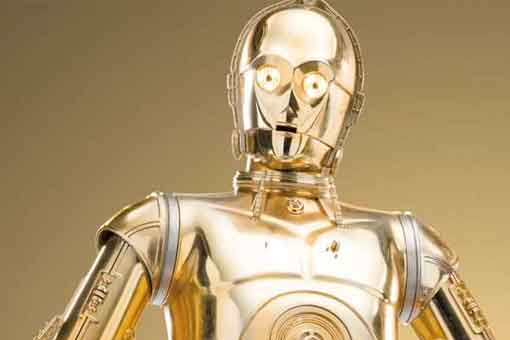
\includegraphics[scale=.2]{imagenes/c3po.jpg}

\end{minipage}

\end{frame}

\begin{frame}{Agentes}

\begin{minipage}{.65\linewidth}

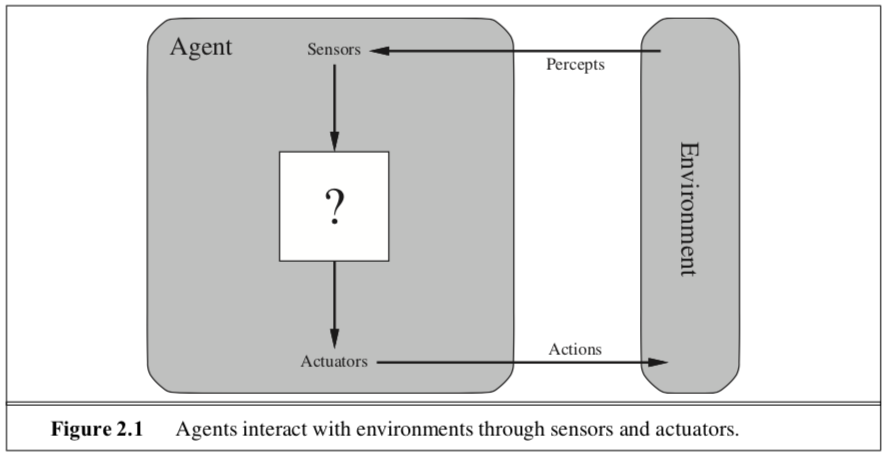
\includegraphics[scale=.2]{imagenes/agente.png}

\

\HandRight\, Programa: Función de sensores a\par actuadores.

\end{minipage}\begin{minipage}{.3\linewidth}

\visible<2->{
\begin{center}
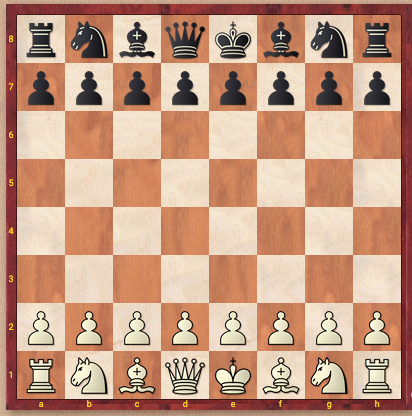
\includegraphics[scale=.15]{imagenes/Tablero1.png}

\includegraphics[scale=.03]{imagenes/arrow.jpg}

{\LARGE e4}
\end{center}
}

\end{minipage}

\end{frame}

\begin{frame}{Agentes y entornos}

\begin{minipage}{0.43\linewidth}
\textbf{Agentes}

\begin{itemize}
\item Dirigidos por tablas
\item Reflejos simples
\item Basados en modelos
\item Basados en objetivos
\item Basados en utilidades
\end{itemize}
\vspace{3\baselineskip}\pause

\end{minipage}\begin{minipage}{0.57\linewidth}
\textbf{Entornos}

\begin{itemize}
\item Completamente observable vs. Parcialmente observable
\item Un agente vs. Multiagentes
\item Determinista vs. Estocástico
\item Episódico vs. Sequencial
\item Estático vs. Dinámico
\item Discreto vs. Continuo
\item Conocido vs. Desconocido
\end{itemize}
\end{minipage}
\end{frame}

\section{El mundo del Wumpus}

\begin{frame}{El mundo del Wumpus (Gregory Yob, 1975)}

\begin{minipage}{.45\linewidth}

\only<1>{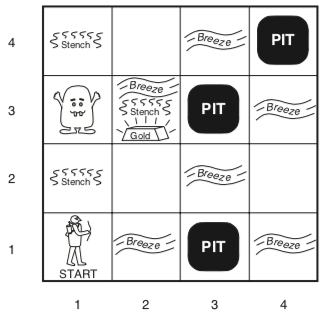
\includegraphics[scale=.55]{imagenes/ejemplo.png}}
\only<2->{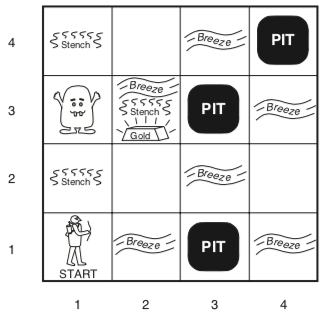
\includegraphics[scale=.37]{imagenes/ejemplo.png}}

\end{minipage}\begin{minipage}{.55\linewidth}

\only<2>{
\begin{block}{Entorno:}
\begin{small}
Una cueva representada por una rejilla $4\times 4$ bordeada por muros. El agente siempre comienza en (0, 0) mirando a la derecha. La ubicación del Wumpus se escoge arbitrariamente de manera uniforme en casillas distintas a la inicial. Cualquier casilla distinta de la inicial puede ser un pozo con probabilidad 0.2.
\end{small}
\end{block}
}

\only<3>{
\begin{block}{Actuadores:} 
\begin{small}
El heroe puede moverse \texttt{adelante} por una casilla (no es posible moverse adelante cuando hay un muro), \texttt{voltearIzquierda} por 90º, o \texttt{voltearDerecha} por 90º. Es posible \texttt{agarrar} el oro cuando este está en la casilla ocupada por el heroe. También puede \texttt{disparar} la flecha en la dirección en que está mirando, la cual seguirá en linea recta hasta golpear un muro. Finalmente, el agente puede \texttt{salir} de la cueva, pero solo desde la casilla inicial.
\end{small}
\end{block}
}

\only<4>{
\begin{block}{Sensores:} 
\begin{small}
El heroe percibe un \texttt{hedor} cuando llega a la casilla donde está el Wumpus o cuando llega a una de las casillas adjacentes (diagonalmente). En las casillas adjacentes a un pozo, percibe una \texttt{brisa}. En el cuadro donde está el oro, percibe un \texttt{brillo}. Cuando se topa con un muro, percibe un \texttt{batacazo}. Finalmente, si el Wumpus muere, el heroe percibe un \texttt{grito} desde cualquier casilla.
\end{small}
\end{block}
}

\only<5>{
\begin{block}{Medida de desempeño:}
\begin{small}
+1000 por salir de la cueva con el oro; -1000 por caer en un pozo o ser comido por el Wumpus; -1 por cada acción y -10 por usar la flecha. El juego termina cuando el heroe muere o sale de la cueva.
\end{small}
\end{block}
}

\end{minipage}

\end{frame}


\begin{frame}{Familiarización}

Intentando encontrar el oro sin morir en el intento...

\

\begin{minipage}{.45\linewidth}

\begin{tikzpicture}

\draw[step=1cm,color=gray] (-2,-2) grid (2,2);

\node at (-1.5,-2.2) {\tiny 0};
\node at (-.5,-2.2) {\tiny 1};
\node at (.5,-2.2) {\tiny 2};
\node at (1.5,-2.2) {\tiny 3};
\node at (-2.2,-1.5) {\tiny 0};
\node at (-2.2,-.5) {\tiny 1};
\node at (-2.2,.5) {\tiny 2};
\node at (-2.2,1.5) {\tiny 3};

\only<1-3>{\node at (-1.5,-1.5) {
\includegraphics[scale=.1]{imagenes/hero.png}};}
\only<4-6>{\node at (-.5,-1.5) {
\includegraphics[scale=.1]{imagenes/hero.png}};}
\only<7-9>{\node at (-1.5,-.5) {\rotatebox[origin=c]{90}{
\includegraphics[scale=.1]{imagenes/hero.png}}};}

\only<2-3>{
\node at (-1.5,-.5) {OK};
\node at (-.5,-1.5) {OK};
}
\only<4>{
\node at (-1.5,-.5) {OK};
\node at (-.8,-1.2) {\tiny OK};
}
\only<5-6>{
\node at (-1.5,-.5) {OK};
\node at (-.8,-1.2) {\tiny OK};
\node at (+.5,-1.5) {\small pozo?};
\node at (-.5,-.5) {\small pozo?};
}
\only<7>{
\node at (-1.8,-.8) {\tiny OK};
\node at (-.5,-1.5) {OK};
\node at (+.5,-1.5) {\small pozo?};
\node at (-.5,-.5) {\small pozo?};
}
\only<8->{
\node at (-1.8,-.8) {\tiny OK};
\node at (-.5,-1.5) {OK};
\node at (+.5,-1.5) {\small pozo};
\node at (-.5,-.5) {OK};
\node at (-1.5,+.5) {\tiny Wumpus};
}

\end{tikzpicture}

\end{minipage}\begin{minipage}{.55\linewidth}

\only<1-3>{
\begin{block}{Sensores}

(\texttt{None}, \texttt{None}, \texttt{None}, \texttt{None}, \texttt{None})

\end{block}
}
\only<4-6>{
\begin{block}{Sensores}

(\texttt{None}, \texttt{brisa}, \texttt{None}, \texttt{None}, \texttt{None})

\end{block}
}
\only<7-9>{
\begin{block}{Sensores}

(\texttt{Hedor}, \texttt{None}, \texttt{None}, \texttt{None}, \texttt{None})

\end{block}
}

\

\only<3>{
\begin{block}{Actuadores}
\texttt{adelante}
\end{block}
}
\only<6>{
\begin{block}{Actuadores}
(\texttt{voltearIzquierda}, \texttt{voltearIzquierda}, \texttt{adelante}, \texttt{voltearDerecha}, \texttt{adelante})
\end{block}
}
\only<9>{
\begin{block}{Actuadores}
\texttt{disparar}
\end{block}
}

\end{minipage}

\end{frame}


\begin{frame}{Propiedades del agente}

\begin{itemize}
\item Toma de decisiones \pause
\item Planeación \pause
\item Representación del conocimiento \pause
\item Inferencias 
\end{itemize}

\end{frame}

\begin{frame}{Taller de ejemplo}

\begin{center}
El mundo del wumpus

\


\includegraphics[scale=.05]{imagenes/Jupyter_logo}

\

\url{https://github.com/Slendercoder/IA_notebooks/tree/master/Teaser/Notebook}
\end{center}

\end{frame}

\begin{frame}{Planeando rutas}

\vspace{-2\baselineskip}

\begin{center}
\begin{tiny}
Heurística 1: Escoger la casilla más cercana al objetivo\hfill Heurística 2: Escoger el camino más corto
\end{tiny}
\end{center}

\begin{minipage}{.45\linewidth}

\begin{tikzpicture}

\draw[step=1cm,color=gray] (-2,-2) grid (2,2);

\node at (-1.5,-2.2) {\tiny 0};
\node at (-.5,-2.2) {\tiny 1};
\node at (.5,-2.2) {\tiny 2};
\node at (1.5,-2.2) {\tiny 3};
\node at (-2.2,-1.5) {\tiny 0};
\node at (-2.2,-.5) {\tiny 1};
\node at (-2.2,.5) {\tiny 2};
\node at (-2.2,1.5) {\tiny 3};

\node at (-1.5,-1.5) {\tiny \alert<9->{Salida}};
\node at (.5,.5) {
\includegraphics[scale=.1]{imagenes/hero.png}};
\node at (1.5,.5) {\tiny Segura};
\node at (.5,-.5) {\tiny \alert<3->{Segura}};
\node at (-.5,-.5) {\tiny \alert<6->{Segura}};
\node at (.5,-1.5) {\tiny Segura};
\node at (-1.5,-.5) {\tiny \alert<8->{Segura}};

\end{tikzpicture}

\end{minipage}\begin{minipage}{.55\linewidth}

\visible<2->{
\begin{center}
\scalebox{0.7}{
\begin{tikzpicture}[level 1/.style={sibling distance=8em},
						level 2/.style={sibling distance=8em}]

\only<2>{
\node[terminal] {Casilla(2,2)}
    child { node[terminal] {Casilla(3,2)} }    
    child { node[terminal] {Casilla(2,1)} }        
;} % end only 2

\only<3>{
\node[terminal] {Casilla(2,2)}
    child { node[vacio] {
\includegraphics[scale=0.05]{imagenes/No_check}} }    
    child { node[terminal] {Casilla(2,1)} }        
;} % end only 3

\only<4>{
\node[terminal] {Casilla(2,2)}
    child { node[vacio] {
\includegraphics[scale=0.05]{imagenes/No_check}} }    
    child { node[terminal] {Casilla(2,1)}
    	child { node[terminal] {Casilla(1,1)} }	
    	child { node[terminal] {Casilla(2,0)} }	
    }    
;} % end only 4

\only<5>{
\node[terminal] {Casilla(2,2)}
    child { node[vacio] {
\includegraphics[scale=0.05]{imagenes/No_check}} }    
    child { node[terminal] {Casilla(2,1)}
    	child { node[terminal] {Casilla(1,1)} }	
    	child { node[terminal] {Casilla(2,0)} 
	    	child { node[terminal] {Casilla(2,1)} }	
	}	
    }    
;} % end only 5

\only<6>{
\node[terminal] {Casilla(2,2)}
    child { node[vacio] {
\includegraphics[scale=0.05]{imagenes/No_check}} }    
    child { node[terminal] {Casilla(2,1)}
    	child { node[terminal] {Casilla(1,1)} }	
    	child { node[vacio] {
\includegraphics[scale=0.05]{imagenes/No_check}} }	
	}	
;} % end only 6

\only<7>{
\node[terminal] {Casilla(2,2)}
    child { node[vacio] {
\includegraphics[scale=0.05]{imagenes/No_check}} }    
    child { node[terminal] {Casilla(2,1)}
    	child { node[terminal] {Casilla(1,1)}  
	    	child { node[terminal] {Casilla(0,1)} }	
	    	child { node[terminal] {Casilla(2,1)} }	
		}	
    	child { node[vacio] {
\includegraphics[scale=0.05]{imagenes/No_check}} }	
	}	
;} % end only 7

\only<8>{
\node[terminal] {Casilla(2,2)}
    child { node[vacio] {
\includegraphics[scale=0.05]{imagenes/No_check}} }    
    child { node[terminal] {Casilla(2,1)}
    	child { node[terminal] {Casilla(1,1)} 
	    	child { node[terminal] {Casilla(0,1)} }	
	    	child { node[vacio] {
\includegraphics[scale=0.05]{imagenes/No_check}} }	
		}	
    	child { node[vacio] {
\includegraphics[scale=0.05]{imagenes/No_check}} }	
	}	
;} % end only 8

\only<9>{
\node[terminal] {Casilla(2,2)}
    child { node[vacio] {
\includegraphics[scale=0.05]{imagenes/No_check}} }    
    child { node[terminal] {Casilla(2,1)}
    	child { node[terminal] {Casilla(1,1)}  
	    	child { node[terminal] {Casilla(0,1)} 
			    child { node[terminal] {Casilla(0,0)} }
			}	
	    	child { node[vacio] {
\includegraphics[scale=0.05]{imagenes/No_check}} }	
		}	
    	child { node[terminal] {Casilla(2,1)} }	
	}	
;} % end only 9

\end{tikzpicture}
}  % end scalebox
\end{center}
} % end visible 2

\end{minipage}

\end{frame}

\begin{frame}{Resumen}

\begin{itemize}
\item La inteligencia de máquina es un tema controversial.
\item El objetivo es construir agentes artificiales que se comporten de manera inteligente.
\item La idea tiene una historia venerable.
\item Clasificación de arquitecturas de agente y de tipos de entorno.
\item Un agente automático que razona y toma decisiones para enfrentar el mundo del Wumpus.
\end{itemize}

\end{frame}

\end{document}

